% \section{Definición}

% Previamente, debemos de llevar a cabo un análisis de los datos y de esta manera obtenemos el esquema conceptual y lógico de la BD. En este tema entre la siguiente fase de \textit{Diseño}, dando como resultado el modelo lógico. Este se trata de uno ya implementado, por eso se dice que es un modelo implementable. 

% En cuanto al proceso de transformación, distinguimos:

% \begin{enumerate}
%     \item Mundo real 
%     \item Datos operativos
%     \item Esquema conceptual
% \end{enumerate}

% En esta etapa se introduce lo que conocemos como \textit{tablas}. En la última fase llevamos a cabo la implementación de esa tabla mediante un lenguaje.

% Definición: Mecanismo formal para representar y manipular la información con la que voy a trabajar. Debe de constar de datos, operaciones y reglas de integridad.

% La necesidad de usar el modelo de datos son:
% \begin{itemize}
%     \item Se usan lenguajes de definición de datos.
%     \item Es de muy bajo nivel.
%     \item Se necesitan niveles superior para su abstracción.
% \end{itemize}

% El objetivo que se tiene es establecer que representen los datos y que los describan de una forma entendible y manipulable. Según ANSI distinguimos tres niveles:
% \begin{itemize}
%     \item Externo
%     \item Conceptual
%     \item Interno
% \end{itemize}

% En cuanto a la clasificación:
% \begin{itemize}
%     \item Basados en registros.
%     \item Basados en objetos.
%     \item Físico.
% \end{itemize}

% Los dos primeros son de nivel externo y conceptual, mientras que el último es de nivel interno.

% \section{Modelo Relacional}

% La información se organiza en tablas: 

% \begin{enumerate}
%     \item La estructura de almacenamiento son las tablas.
%     \item Integridad.
%     \item Consulta y Manipulación.
% \end{enumerate}

% Esta tabla es a nivel lógico, en cuanto al nivel físico depende de varias estructuras, como son las listas enlazadas,...

% Elementos a conocer:
% \begin{itemize}
%     \item Atributo.
%     \item Dominio: rango de valores que puede tomar (enteros, letras,...)
%     \item Relación: Se conoce como cualquier subconjunto del producto cartesiano $D_1 \times D_2 \times ... D_n$. En este caso a relación se refiere a la tabla. Se denota como $R(A_1..A_n)$. De esta manera conseguimos todos los valores que pueden tomar y de aquí sacamos los datos (solo a nivel teórico).
%     \item Tupla: filas de la tabla.
%     \item Cardinalidad de una relación: número de tuplas.
%     \item Esquema de una relación R: Atributos de la relación junto a su dominio.
%     \item Grado de una relación: Número de atributos. Aunque se supone que es invariable, esto depende ya que se puede modificar.
%     \item Instancia de una relación: datos que tengo en un determinado momento.
%     \item Esquema de la BD: colección de esquemas de relaciones junto con las restricciones de integridad.
%     \item Instancia o estado de una BD: colección de instancias de relaciones que verifican las condiciones de integridad.
%     \item BD relaciones: instancia de la BD junto con su esquema.
% \end{itemize}

% \subsubsection*{Condición de Normalización}

% \begin{itemize}
%     \item Todos los valores de los atributos de una relación son atómicos\footnote{No se pueden dividir más}.
%     \item Valor atómico es un valor no estructurado.
%     \item Cuando una relación cumple la condición de normalización se dice que está en Primera Forma Normal.
% \end{itemize}

% \subsubsection*{Consecuencias}

% \begin{itemize}
%     \item No hay valores tipo conjunto.
%     \item No hay valores tipo registro.
%     \item No hay valores tipo tablas.
% \end{itemize}

% \subsubsection*{Problema}

% Todas las representaciones son extensivas, no se puede representar información del tipo “el valor del atributo asignaturas de un alumno es: FBD, ALG, LD”.


% \subsubsection*{Consecuencias de la definición}

% \begin{itemize}
%     \item No hay tuplas duplicadas:
%     \begin{itemize}
%         \item Por la definición conjuntista de relación.
%     \end{itemize}
%     \item No hay orden en las filas ni en los atributos:
%     \begin{itemize}
%         \item Al no estar ordenados ni los atributos ni las filas (conjuntos) el acceso es por nombre de atributo y valor.
%     \end{itemize}
%     \item Varias instancias representan la misma relación.
% \end{itemize}

% \begin{table}[h!]
% \centering
% \begin{tabular}{|c|c|c|c|c|}
% \hline
% A & B & C & D & E \\ \hline
% a1 & b1 & c1 & d1 & e1 \\ \hline
% a1 & b2 & c2 & d2 & e1 \\ \hline
% a2 & b1 & c3 & d3 & e1 \\ \hline
% a2 & b1 & c4 & d3 & e1 \\ \hline
% a3 & b2 & c5 & d1 & e1 \\ \hline
% \end{tabular}
% \end{table}

% \begin{table}[h!]
% \centering
% \begin{tabular}{|c|c|c|c|c|}
% \hline
% A & B & C & D & E \\ \hline
% a2 & b1 & c4 & d3 & e1 \\ \hline
% a2 & b1 & c3 & d3 & e1 \\ \hline
% a1 & b2 & c2 & d2 & e1 \\ \hline
% a3 & b2 & c5 & d1 & e1 \\ \hline
% a1 & b1 & c1 & d1 & e1 \\ \hline
% \end{tabular}
% \end{table}

% En cuanto a las representaciones podemos distinguir:
% \begin{itemize}
%     \item Representación física: Archivos, registros y campos.
%     \item Representación intuitiva: Tabla, filas y columnas.
%     \item Modelo matemático: Relación, tuplas y atributos.
% \end{itemize}

% \section{El modelo de datos relacional. ED. Integridad}
% \subsection{La estructura de datos relacional}

% \subsection*{Notación a utilizar}
% \begin{itemize}
%     \item Relación: R, S, T....
%     \item Atributos: A, B, ...
%     \item Esquema de relación: R[A1, A2, ..., An]
%     \item Instancia de relación R: r
%     \item Tuplas de una instancia: x1, x2, ..., $\in$ r
%     \item Valor de un atributo Ai en una tupla xj: xj[Ai] ó Aij
% \end{itemize}

% \subsection*{Valores nulos}
% \begin{itemize}
%     \item Algunas veces no se conoce el valor de un atributo para una determinada tupla. En esos casos a ese atributo de esa tupla se le asigna un valor nulo (NULL).
%     \item Un valor nulo puede ser:
%     \begin{itemize}
%         \item Un valor desconocido.
%         \item Un atributo no aplicable.
%     \end{itemize}
%     \item En cualquier caso, ese valor es un valor más de todos los dominios de la base de datos.
% \end{itemize}

% \subsection{Restricciones o reglas de integridad}

% \begin{itemize}
%     \item Son condiciones para preservar la semántica de una base de datos.
%     \item Específicas del problema:
%     \begin{itemize}
%         \item $0 \leq \text{edad} \leq 100$
%         \item $\text{créditos} > 0$
%         \item $\text{carácter} \in \{\text{'troncal', 'obligatoria', 'optativa', ...}\}$
%     \end{itemize}
%     \item Propias del papel de los atributos en el esquema:
%     \begin{itemize}
%         \item $\text{imparte.NRP} \in \text{profesor.NRP}$ (un profesor inexistente no puede impartir una asignatura)
%         \item $\text{cod\_asig} \neq \text{nulo}$ (siempre debe conocerse el código de una asignatura)
%     \end{itemize}
% \end{itemize}

% \subsection*{Superclaves y claves (candidatas y primarias)}
% \begin{itemize}
%     \item Superclave: Cualquier conjunto de atributos que identifica unívocamente a cada tupla de una relación.
%     \item Clave de una relación: superclave minimal.
%     \item Por ejemplo, en la relación Asignaturas:
%     \begin{itemize}
%         \item El conjunto de atributos \{Cod\_Asig, Nombre\} identifica unívocamente cada tupla.
%         \item Sin embargo, no es minimal y no puede considerarse como una clave.
%         \item Cod\_Asig por sí sola, es una clave.
%     \end{itemize}
% \end{itemize}

% \begin{itemize}
%     \item En una relación dada puede que más de un conjunto de atributos puedan ser elegidos como clave. Estos conjuntos de atributos se llaman claves candidatas.
%     \item Cuando hay más de una clave candidata, hay que seleccionar una como principal. Esta clave recibe el nombre de clave primaria de la tabla.
%     \item Criterio de selección: Tamaño, significado, \textbf{capacidad para recordarla}\footnote{Ejemplo de ello, es cuando vas a secretaría a preguntar por algo, donde te preguntan por tu DNI, en vez de Nº de expediente.}, fusión con otras tablas, etc.
% \end{itemize}

% \subsubsection*{Clave candidata y primaria (definición formal)}

% \begin{itemize}
%     \item Sea R[A1, A2, ..., An], CC $\subseteq \{A1, A2, ..., An\}$ se denomina clave candidata si y solo si:
%         \begin{itemize}
%             \item \textbf{Unicidad}: $\forall r$ instancia de R y $\forall t1, t2 \in r$ con $t1 \neq t2 \Rightarrow t1[CC] \neq t2[CC]$\footnote{No puede coincidir dos tuplas distintas.}
%             \item \textbf{Minimalidad}: No existe CC' $\subseteq$ CC que verifique la unicidad.
%         \end{itemize}
%         \item Una clave candidata es un atributo o conjunto de atributos que identifican a cada tupla en la relación y que, además, no existe un subconjunto de ellos que también identifiquen a cada tupla de la relación.
%         \item Una clave primaria es una clave candidata elegida por el diseñador.
%         \item Si CC verifica la unicidad pero no la minimalidad se denomina superclave.
%         \item Completamos la notación para describir una relación, subrayando los atributos que forman su clave primaria etiquetándolos con CP. Si existen otras claves candidatas también se subrayan etiquetando el subrayado con CC:
%         \begin{itemize}
%             \item Socio (\underline{\#Socio\textsubscript{CP}}, \underline{DNI\textsubscript{CC}}, Nombre, Dirección)\footnote{En este caso estamos denotando como se referencia en la práctica.}
%         \end{itemize}
% \end{itemize}

% \subsubsection*{Claves externas}

% \begin{itemize}
%     \item Conjunto de atributos en una relación que es una clave en otra (o incluso en la misma) relación.
%     \item Podemos ver una clave externa como un conjunto de atributos de una relación cuyos valores en las tuplas deben coincidir con los valores de la clave primaria de las tuplas de la otra relación.
% \end{itemize}

% \subsubsection*{Claves externas}

% \begin{itemize}
%     \item Consideramos una relación R (relación que referencia) y un subconjunto de atributos de su esquema CE (clave externa); y una relación S (relación referenciada) cuya clave primaria CP coincide con CE.
%     \item Si CE es una clave externa de R que referencia a CP en S, entonces: $\forall t \in r, \exists t' \in s$ tal que $t[CE] = t'[CP]$, donde $r$ y $s$ son las instancias de R y S en la base de datos.
%     \item Eventualmente, R y S pueden ser la misma relación.
% \end{itemize}

% \begin{itemize}
%     \item Ejemplo: Imparte (NRP, Cod\_Asig) referencia a Profesor (NRP).
% \end{itemize}

% \subsubsection*{Dominio activo}

% \begin{itemize}
%     \item Subconjunto de valores del dominio de un atributo de una relación que está presente en la instancia de la relación\footnote{Es decir, en un momento dado.}.
%     \item Dada una relación R, su instancia r y un atributo A de R, el dominio activo de A es el siguiente conjunto:
%     \[
%     \{a \mid \exists t \in r \text{ tal que } t[A] = a\}
%     \]
%     \item Podemos extender el concepto de dominio activo a un conjunto de atributos.
%     \item Dada una relación R, su instancia r y un subconjunto de atributos CA de R, el dominio activo de CA es el siguiente conjunto:
%     \[
%     \{(a_1, a_2, \ldots, a_n) \mid \exists t \in r \text{ tal que } t[CA] = (a_1, a_2, \ldots, a_n)\}
%     \]
%     \item Las claves externas establecen relaciones de inclusión entre los dominios activos de la clave externa y la clave referenciada.
% \end{itemize}

% \begin{itemize}
%     \item Puede haber más de una clave externa en una relación.
%     \item Puede haber una clave externa a la clave primaria de la propia relación\footnote{No puede haber  dos claves en la misma sección que se llamen igual, por lo que si en una relacion nos encontramos con dos DNI, debemos de denotar uno de manera distinta, o bien usar una notación distinta.}.
%     \item El resultado de que haya CE con una misma relación es el hecho de la \textit{fusión de tablas}.
% \end{itemize}

% \subsection*{Conceptos generales}
% \begin{itemize}
%     \item Condiciones de integridad:
%     \begin{itemize}
%         \item Normas que mantienen la corrección semántica de una base de datos.
%     \end{itemize}
%     \item Nos centramos en la integridad genérica: depende del papel que juegue un atributo en el diseño de la tabla:
%     \begin{itemize}
%         \item Son metarreglas: generan reglas de integridad aplicadas a una base de datos concreta.
%         \item Existen la integridad de entidad y la integridad referencial.
%     \end{itemize}
% \end{itemize}

% \subsubsection*{Integridad de entidad}
% \begin{itemize}
%     \item No se debe permitir que una entidad sea representada en la base de datos si no se tiene una \textbf{información completa} de los atributos que son clave primaria de la entidad.
%     \item Un atributo que forma parte de la clave primaria de una tupla en una relación, \textbf{no puede tener un valor nulo}\footnote{Esto define la integridad de la tabla.}.
% \end{itemize}

% \subsubsection*{Integridad referencial}
% \begin{itemize}
%     \item Una base de datos en la que \textbf{todos los valores no nulos de una clave externa referencian valores reales de la clave referenciada} en la otra relación, cumple la regla de integridad referencial. Si esto se cumple, estamos cumpliendo con la regla de \textit{integridad referencial}.
%     \item Si una relación incluye una clave externa conectada a una clave primaria, el valor de la clave externa debe ser, o bien igual a un valor ya existente en el dominio activo de la clave primaria, o bien completamente nulo (si la semántica lo permite).
%     \item La integridad referencial mantiene las conexiones en las bases de datos relacionales.
% \end{itemize}

% \subsection*{Restricciones del SGBD}

% EL SGBD debe encargarse de mantener las siguientes restricciones:
% \begin{itemize}
%     \item La unicidad de la clave primaria y de las claves candidatas:
%     \begin{itemize}
%         \item Frente a operaciones de inserción y actualización, el SGBD debe rechazar los valores introducidos que sean iguales a los presentes en la BD para los atributos que el diseñador ha definido como clave primaria y como claves candidatas.
%     \end{itemize}
%     \item La integridad de identidad:
%     \begin{itemize}
%         \item Frente a operaciones de inserción y actualización, el SGBD debe rechazar las modificaciones que asignen un valor NULO a algún atributo de la clave primaria.
%     \end{itemize}
% \end{itemize}

% \begin{itemize}
%     \item La integridad referencial:
%     \begin{itemize}
%         \item En inserciones:
%         \begin{itemize}
%             \item Rechazar la tupla insertada si el valor de la clave externa no concuerda en la relación referenciada para alguna tupla en el valor su clave primaria, es decir, si no es nulo o bien no existe.
%             \item Si el valor para la clave externa es NULO y el diseño no lo permite, habrá que \textit{rechazar} también esa inserción.
%         \end{itemize}
%         \item En borrados:
%         \begin{itemize}
%             \item Si se borra la clave primaria en la relación referenciada, el diseñador puede establecer en el SGBD una de las siguientes alternativas de actuación:
%             \begin{itemize}
%                 \item Rechazar el borrado de la tupla.
%                 \item Eliminar en cadena todas las tuplas que la referencian.
%                 \item Poner valor nulo en la clave externa de todas esas tuplas.
%             \end{itemize}
%         \end{itemize}
%         \item En actualizaciones:
%         \begin{itemize}
%             \item Si se actualiza la clave externa, actuar con el nuevo valor actualizado como en el caso de inserción.
%             \item Si se actualiza la clave primaria de la relación referenciada y el antiguo valor estaba referenciado en alguna relación, actuar como en el caso de borrado.
%         \end{itemize}
%     \end{itemize}
% \end{itemize}

% \section{Otros modelos de datos}

% \subsection{Modelo jerárquico}

% Fue el primero en implementarse físicamente:
% \begin{itemize}
%     \item Nivel externo: aplicaciones Cobol o lenguaje del sistema.
%     \item No había interactividad:
%     \begin{itemize}
%         \item Carecía de un lenguaje de consulta.
%     \end{itemize}
%     \item Estructura de datos básica:
%     \begin{itemize}
%         \item Árbol:
%         \begin{itemize}
%             \item Registro maestro: raíz.
%             \item Registros secundarios: dependen de los anteriores.
%         \end{itemize}
%     \end{itemize}
%     \begin{itemize}
%         \item La BD es una colección de instancias de árboles.
%         \item Esta estructura plasma de forma muy directa:
%         \begin{itemize}
%             \item Relaciones muchos a uno.
%             \item Relaciones uno a uno.
%         \end{itemize}
%         \item Para relaciones muchos a muchos:
%         \begin{itemize}
%             \item Hay que duplicar toda la información sobre las entidades involucradas.
%         \end{itemize}
%     \end{itemize}
% \end{itemize}

\section{Relaciones de Ejercicios T3}

\subsection{Relación A}

\begin{enumerate}[label=\textbf{\arabic*.}, itemsep=0.5em]
    \item ¿Cuándo aparece el concepto de modelo de datos? ¿Por qué?
    
    El concepto de modelo de datos surge en la década de 1970 debido a la necesidad de estructurar la información en bases de datos de manera más eficiente y organizada. Antes de esto, los sistemas de gestión de datos utilizaban enfoques desordenados y dependientes de estructuras jerárquicas o de redes, lo que dificultaba la manipulación, recuperación y mantenimiento de la información. Con la llegada del modelo relacional de Edgar F. Codd, se estableció una base teórica sólida para la gestión de datos, promoviendo su independencia del hardware y los programas específicos.

    \item Diferencias entre los modelos de datos semánticos y los modelos de datos implementables.
    
    Modelos de datos semánticos: Representan la información a un nivel conceptual, describiendo cómo los datos se relacionan entre sí en el mundo real. Se enfocan en el significado de los datos y en su estructura lógica, sin preocuparse por su almacenamiento físico. Un ejemplo es el Modelo Entidad-Relación (E-R).

    Modelos de datos implementables: Son aquellos diseñados para su almacenamiento y gestión en un Sistema de Gestión de Bases de Datos (SGBD). Se derivan de los modelos semánticos y adaptan los datos a estructuras que pueden ser manejadas por un sistema informático, como tablas en el modelo relacional.

    \item Define entidad y proporciona algún ejemplo. Distinguir entre conjunto de entidades y entidad concreta.

        Entidad: Es cualquier objeto del mundo real que puede identificarse de manera única y que posee atributos que lo describen. Puede ser una persona, un lugar, un evento o un concepto.

        Ejemplo: Un Estudiante.

        Conjunto de entidades: Representa el grupo de todas las entidades del mismo tipo. En este caso, todos los estudiantes de una universidad.

        Entidad concreta: Se refiere a una instancia específica dentro del conjunto de entidades. Ejemplo: Juan Pérez, que es un estudiante concreto dentro del grupo de estudiantes.

    \item Para el ejemplo de entidad antes definida, define sus atributos y proporciona un ejemplo. Identificar la clave primaria de ésta.

        Atributos del Estudiante: Nombre, Apellido, Matrícula, Fecha de nacimiento, Carrera.

        Ejemplo de instancia:

            Nombre: Juan

            Apellido: Pérez

            Matrícula: 12345

            Fecha de nacimiento: 01/01/2000

            Carrera: Ingeniería Informática

        Clave primaria: Matrícula. Este atributo es único para cada estudiante y permite identificarlo sin ambigüedad.

    \item Poner un ejemplo de atributo compuesto relacionado con la entidad definida antes.

        Un atributo compuesto es aquel que puede dividirse en subcomponentes con significado propio.

        Para la entidad Estudiante, un atributo compuesto podría ser la Dirección, que se divide en:

            \begin{itemize}
                \item Calle
                \item Número
                \item Ciudad
                \item Código postal
            \end{itemize}

        Ejemplo: ``Av. Siempre Viva, 742, Huéscar, 1234''.
        \item Definir relación y dar un ejemplo que involucre a la entidad antes definida.  
        Una relación es la asociación entre dos o más entidades. Representa la forma en que los objetos del mundo real están conectados.  
        
        Ejemplo: La entidad \inlinecode{Estudiante} puede estar relacionada con la entidad \inlinecode{Curso} mediante la relación \inlinecode{Inscrito\_en}, indicando en qué cursos está matriculado cada estudiante.
        
        \item Dar un ejemplo de relación de grado mayor que dos, referente a la entidad antes definida.  
        Una relación de grado mayor que dos involucra tres o más entidades.  
        
        Ejemplo: La relación \inlinecode{Evalúa} entre las entidades \inlinecode{Estudiante}, \inlinecode{Profesor} y \inlinecode{Curso}, donde un profesor evalúa a un estudiante en un curso específico.
        
        \item Definir cardinalidad máxima y mínima y dar dos ejemplos: uno referente a una relación uno a muchos y otro referente a una relación muchos a muchos.  
        La cardinalidad mínima indica el número mínimo de veces que una entidad puede participar en una relación. La cardinalidad máxima define el número máximo de veces que una entidad puede estar en una relación.
        
        Ejemplos:  
        \begin{itemize}
            \item Relación uno a muchos:
            \begin{itemize}
                \item Un \inlinecode{Profesor} puede impartir muchos \inlinecode{Cursos}, pero cada curso solo tiene un profesor.
                \item Cardinalidad: (\inlinecode{Profesor} 1:N \inlinecode{Curso}).
            \end{itemize}
            \item Relación muchos a muchos:
            \begin{itemize}
                \item Un \inlinecode{Estudiante} puede inscribirse en varios \inlinecode{Cursos} y un curso puede tener varios estudiantes.
                \item Cardinalidad: (\inlinecode{Estudiante} M:N \inlinecode{Curso}).
            \end{itemize}
        \end{itemize}
        \item Definir entidad débil, dar dos ejemplos diferentes de los estudiados en clase.  
        Una entidad débil es aquella que no puede identificarse de manera única sin la ayuda de otra entidad, llamada entidad fuerte, de la que depende.  
        
        \begin{itemize}
            \item \inlinecode{Historial\_Médico}, que depende de la entidad fuerte \inlinecode{Paciente}.
            \item \inlinecode{Dependiente}, que depende de la entidad fuerte \inlinecode{Empleado} en una empresa.
        \end{itemize}
        
        \item Distinguir mediante ejemplos los conceptos de entidad débil y de relación uno a muchos.  
        \begin{itemize}
            \item Entidad débil:
            \begin{itemize}
                \item Un \inlinecode{Dependiente} no puede existir sin un \inlinecode{Empleado}, ya que su identificación depende de este.
            \end{itemize}
            \item Relación uno a muchos:
            \begin{itemize}
                \item Un \inlinecode{Profesor} puede impartir varios \inlinecode{Cursos}, pero un curso solo tiene un profesor. Aquí, ambas entidades son independientes, a diferencia de la entidad débil.
            \end{itemize}
        \end{itemize}
        
        \item Establecer la conexión entre el concepto de entidad débil y el de atributo compuesto multivaluado. Ilustrar esta idea mediante dos ejemplos. \\\\ 
        Una entidad débil puede representar información que en algunos casos podría modelarse como un atributo compuesto multivaluado, dependiendo del nivel de detalle requerido.
        
        \begin{itemize}
            \item Entidad débil: Un \inlinecode{Historial\_Médico} es una entidad que almacena múltiples registros de un \inlinecode{Paciente}.
            \begin{itemize}
                \item Alternativa: Un atributo compuesto multivaluado \inlinecode{Historial\_Médico} en la entidad \inlinecode{Paciente}, con los campos \inlinecode{Fecha, Diagnóstico, Tratamiento}.
            \end{itemize}
            \item Entidad débil: Un \inlinecode{Dependiente} de un \inlinecode{Empleado} (hijo, cónyuge).
            \begin{itemize}
                \item Alternativa: Un atributo compuesto multivaluado \inlinecode{Dependientes} en la entidad \inlinecode{Empleado} con los campos \inlinecode{Nombre, Relación, Fecha\_Nacimiento}.
            \end{itemize}
        \end{itemize}
        
        \item Define el concepto de subtipo, poner dos ejemplos que no se hayan explicado en clase.  
        Un subtipo es una especialización de una entidad que hereda sus atributos y puede agregar otros específicos.  
        
        \begin{itemize}
            \item \inlinecode{Vehículo} con los subtipos \inlinecode{Coche} y \inlinecode{Motocicleta}.
            \item \inlinecode{Dispositivo\_Electrónico} con los subtipos \inlinecode{Smartphone} y \inlinecode{Tablet}.
        \end{itemize}
        
        \item Define el concepto de herencia. ¿Cómo se relaciona con el caso anterior?  \\\\
        La herencia en bases de datos es el mecanismo mediante el cual un subtipo hereda atributos y relaciones de una entidad general.  
        
        Se relaciona con los subtipos porque estos aplican herencia para compartir atributos comunes. Por ejemplo, \inlinecode{Vehículo} tiene un atributo \inlinecode{Matrícula}, que es heredado por \inlinecode{Coche} y \inlinecode{Motocicleta}.
        
    % \item Explicar la diferencia entre la relación TIENE-UN y la relación ES-UN, y poner un ejemplo de cada una de ellas.
    % \item Poner un ejemplo mediante un diagrama entidad/relación de cada una de las siguientes situaciones:
    % \begin{enumerate}
    %     \item Relación con atributos uno a muchos.
    %     \item Relación involutiva muchos a muchos.
    %     \item Una relación ternaria con algún atributo adicional.
    %     \item Una relación ES-UN donde las subclases tengan atributos adicionales.
    %     \item Entidades fuerte y débil donde esta última se conecte con otras entidades del diagrama.
    % \end{enumerate}
    % \item Decidir de forma razonada cuándo se debe incluir una entidad nueva junto con una relación, o un atributo en cada uno de los siguientes casos. En el caso de que se trate de una entidad con una relación, especificar las características de la misma:
    % \begin{enumerate}
    %     \item La fecha de edición de un libro.
    %     \item Los autores de un libro.
    %     \item El título de una película.
    %     \item Los actores de una película.
    %     \item La valoración psicológica de un alumno.
    %     \item La descripción de un accidente.
    %     \item Los cuartos de baño que tiene un apartamento.
    %     \item El programa de una asignatura.
    %     \item El responsable de una investigación criminal.
    %     \item La fecha de un crimen.
    %     \item Los datos laborales de los trabajadores.
    %     \item El horario de una asignatura.
    % \end{enumerate}
    % \item Poner un ejemplo mediante el diagrama entidad/relación de cada una de las siguientes situaciones. Pasar a tablas el resultado, indicando la clave primaria de la tabla resultante.
    % \begin{enumerate}
    %     \item Una relación ternaria con algún atributo adicional.
    %     \item Una relación ES-UN, donde las subclases tengan atributos adicionales.
    %     \item Entidades subordinante y subordinada.
    %     \item Tipo y subtipo con herencia de propiedades.
    %     \item Relación con atributos uno a muchos.
    %     \item Relación involutiva muchos a muchos.
    % \end{enumerate}
    % \item Poner ejemplos de los distintos casos que aparecen cuando se pasa de una conexión en el modelo E/R a una tabla en el modelo relacional. Estudiar las distintas posibilidades de clave primaria que pueden aparecer.
    % \item ¿Por qué crees que los modelos basados en grafos no mantienen realmente la independencia física?
    % \item ¿Qué crees que significa la afirmación de que el modelo relacional es simétrico con respecto a las relaciones muchos a muchos?
    % \item Poner tres ejemplos de conexiones en el modelo E/R que no se trasladen bien al modelo relacional.

    \item Explicar la diferencia entre la relación TIENE-UN y la relación ES-UN, y poner un ejemplo de cada una de ellas. \\\\ 
    La relación \textbf{TIENE-UN} indica que una entidad posee otra entidad o atributo, pero ambas siguen siendo entidades distintas. En cambio, la relación \textbf{ES-UN} representa una jerarquía de especialización donde una entidad es un subtipo de otra y hereda sus atributos.

    \begin{itemize}
        \item Ejemplo de \textbf{TIENE-UN}: Una entidad \texttt{Coche} tiene un \texttt{Motor}. Aquí, \texttt{Motor} es una entidad independiente que se relaciona con \texttt{Coche}.
        \item Ejemplo de \textbf{ES-UN}: Una entidad \texttt{Empleado} puede especializarse en \texttt{Ingeniero} y \texttt{Administrativo}. En este caso, \texttt{Ingeniero} y \texttt{Administrativo} heredan atributos de \texttt{Empleado}.
    \end{itemize}

    \item Poner un ejemplo mediante un diagrama entidad/relación de cada una de las siguientes situaciones:
    \begin{enumerate}
        \item Relación con atributos uno a muchos.
        \item Relación involutiva muchos a muchos.
        \item Una relación ternaria con algún atributo adicional.
        \item Una relación ES-UN donde las subclases tengan atributos adicionales.
        \item Entidades fuerte y débil donde esta última se conecte con otras entidades del diagrama.
    \end{enumerate}

    \begin{figure}[H]
        \centering
        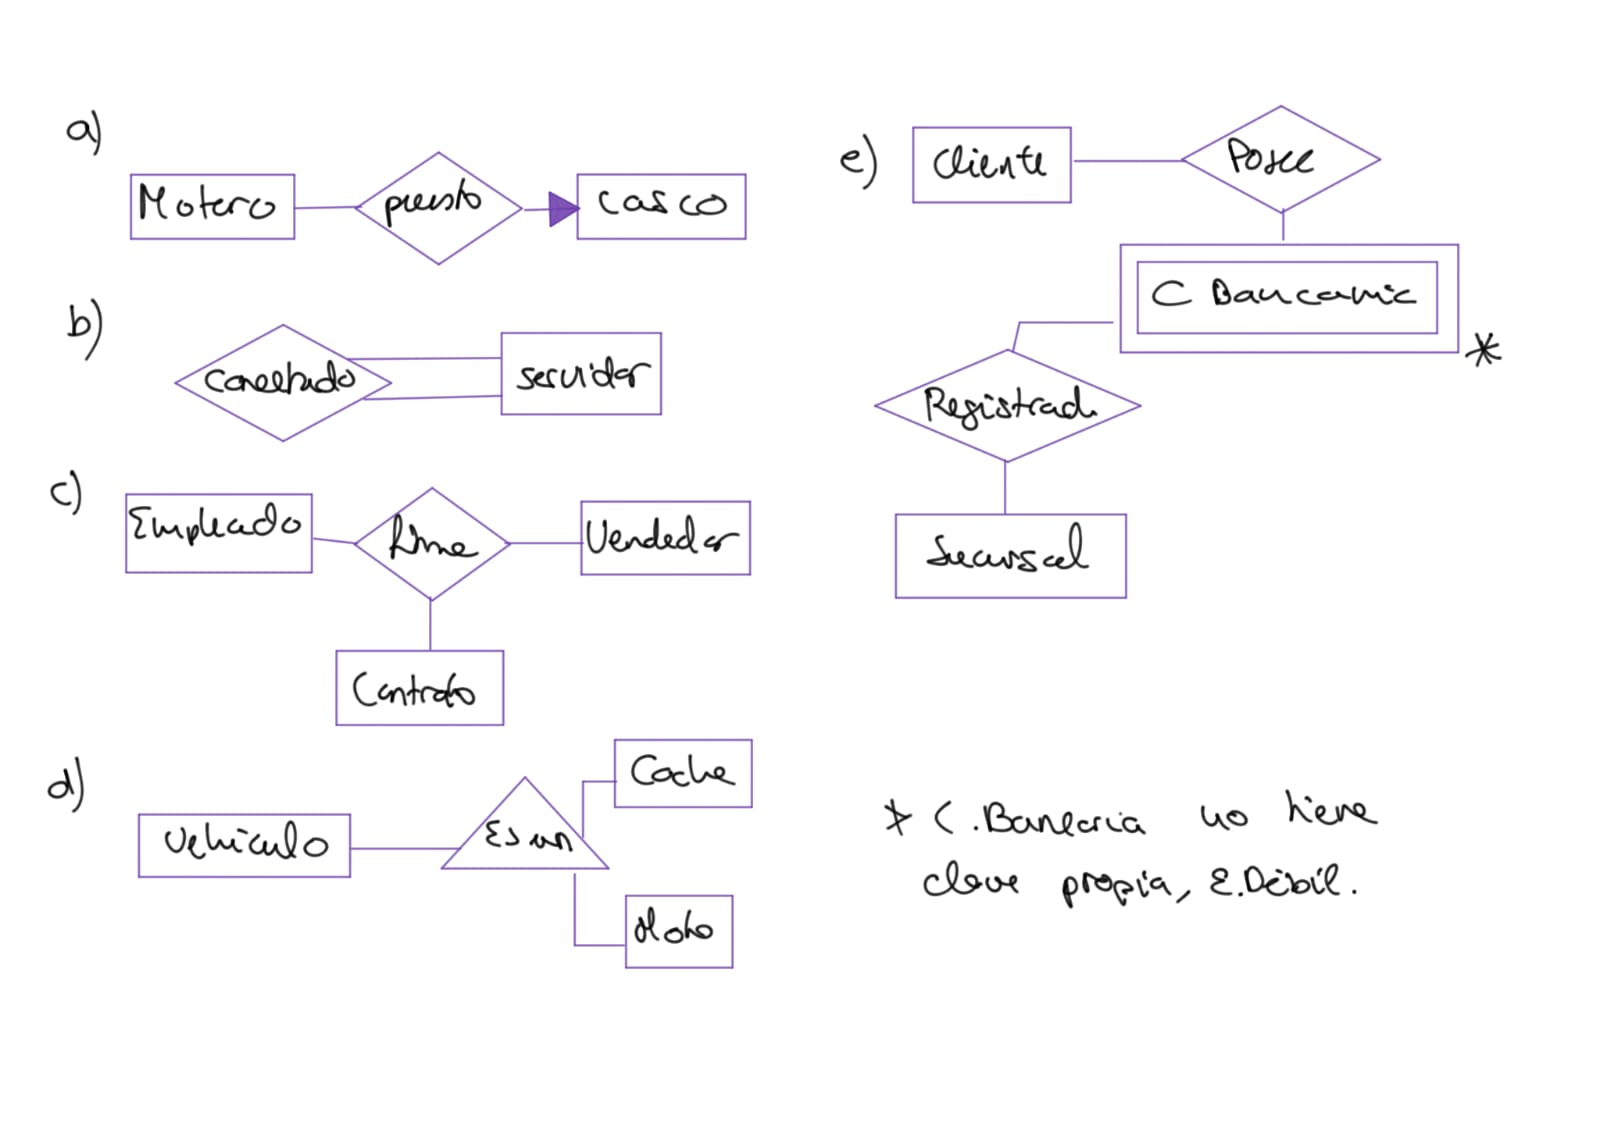
\includegraphics[width=1\textwidth]{images/ej15Rel3A.jpeg}
        \caption{Resolución del ejercicio 15 de la relación 3A. \textit{Nota: Se han obviado los atributos, ya que se supone que son triviales.}}
        \label{fig:diagrama_1}
    \end{figure}

    

    \item Decidir de forma razonada cuándo se debe incluir una entidad nueva junto con una relación, o un atributo en cada uno de los siguientes casos.
    \begin{enumerate}
        \item La fecha de edición de un libro.  
        \textbf{Atributo}, ya que es una propiedad intrínseca del libro.

        \item Los autores de un libro.  
        \textbf{Entidad con relación}, porque un autor puede escribir varios libros y un libro puede tener varios autores (relación muchos a muchos).

        \item El título de una película.  
        \textbf{Atributo}, ya que es una característica única de la película.

        \item Los actores de una película.  
        \textbf{Entidad con relación}, ya que un actor puede participar en varias películas y una película puede tener varios actores.

        \item La valoración psicológica de un alumno.  
        \textbf{Entidad con relación}, porque puede haber múltiples valoraciones en diferentes fechas, asociadas a cada alumno.

        \item La descripción de un accidente.  
        \textbf{Atributo}, ya que es una información específica de la entidad \texttt{Accidente}.

        \item Los cuartos de baño que tiene un apartamento.  
        \textbf{Atributo}, porque es una propiedad fija del apartamento.

        \item El programa de una asignatura.  
        \textbf{Entidad con relación}, porque el programa puede cambiar con el tiempo y necesita un historial.

        \item El responsable de una investigación criminal.  
        \textbf{Entidad con relación}, ya que un investigador puede encargarse de varias investigaciones.

        \item La fecha de un crimen.  
        \textbf{Atributo}, ya que es una característica propia de la entidad \texttt{Crimen}.

        \item Los datos laborales de los trabajadores.  
        \textbf{Entidad con relación}, porque pueden cambiar con el tiempo (salario, cargo, antigüedad, etc.).

        \item El horario de una asignatura.  
        \textbf{Entidad con relación}, ya que una asignatura puede tener múltiples horarios en distintos semestres.
    \end{enumerate}

    \item Poner un ejemplo mediante el diagrama entidad/relación de cada una de las siguientes situaciones y pasar a tablas el resultado, indicando la clave primaria de la tabla resultante.
    \begin{enumerate}
        \item Una relación ternaria con algún atributo adicional.
        Similar al ejercicio 15 c) de la relación 3A, pero con un atributo adicional \texttt{Fecha\_Inscripción}.
        \item Una relación ES-UN, donde las subclases tengan atributos adicionales.
        Similar al ejercicio 15 d) de la relación 3A, pero con un atributo adicional.

        \item Entidades subordinante y subordinada.
        \item Tipo y subtipo con herencia de propiedades.
        \item Relación con atributos uno a muchos.
        Similar al ejercicio 15 a) de la relación 3A, pero con un atributo adicional.
        \item Relación involutiva muchos a muchos.
        Similar al ejercicio 15 b) de la relación 3A.
    \end{enumerate}

    \begin{figure}[H]
        \centering
        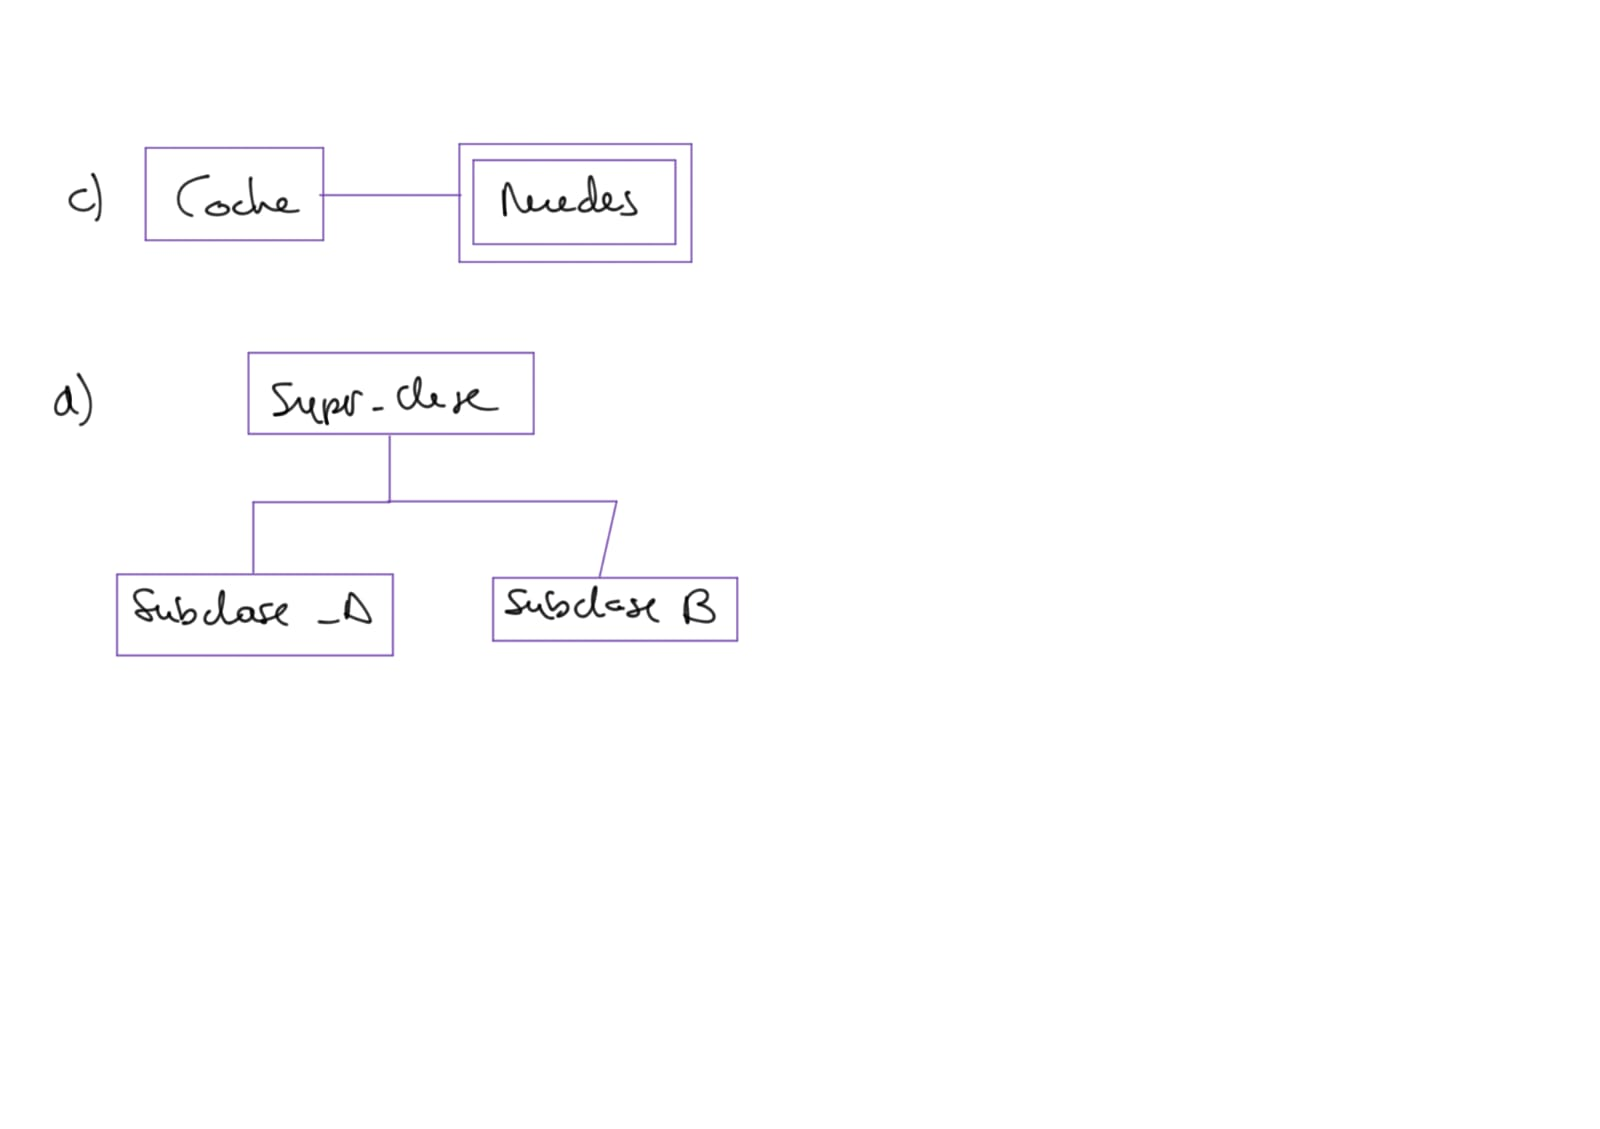
\includegraphics[width=1\textwidth]{images/ej17Rel3A.jpeg}
        \caption{Resolución del ejercicio 17 de la relación 3A. \textit{Nota: Se han obviado los atributos, ya que se supone que son triviales.}}
        \label{fig:diagrama_2}
    \end{figure}


    \textit{(Nota: Se requiere un diagrama E/R para representar gráficamente estas situaciones y su transformación en tablas relacionales.)}

    \item Poner ejemplos de los distintos casos que aparecen cuando se pasa de una conexión en el modelo E/R a una tabla en el modelo relacional. Estudiar las distintas posibilidades de clave primaria que pueden aparecer.  
    Los casos principales son:
    \begin{itemize}
        \item Relación uno a uno: La clave primaria de una entidad puede actuar como clave foránea en la otra.
        \item Relación uno a muchos: La clave primaria de la entidad del lado "uno" se usa como clave foránea en la entidad del lado "muchos".
        \item Relación muchos a muchos: Se crea una tabla intermedia con claves foráneas de ambas entidades como clave primaria compuesta.
    \end{itemize}

    \item ¿Por qué crees que los modelos basados en grafos no mantienen realmente la independencia física?  \\\\
    Porque la estructura del almacenamiento en un modelo basado en grafos depende directamente de la forma en que se almacenan los nodos y las relaciones, lo que afecta el rendimiento según la implementación en la base de datos subyacente.

    \item ¿Qué crees que significa la afirmación de que el modelo relacional es simétrico con respecto a las relaciones muchos a muchos?  \\\\
    Significa que las relaciones muchos a muchos en el modelo relacional se representan de manera uniforme mediante una tabla intermedia, sin importar el tipo de entidades involucradas. Esto garantiza una representación consistente de las relaciones complejas.

    \item Poner tres ejemplos de conexiones en el modelo E/R que no se trasladen bien al modelo relacional.  
    \begin{itemize}
        \item Jerarquías de herencia: Requieren estrategias como el uso de una tabla por subtipo o una tabla con un campo que indique el tipo.
        \item Relaciones recursivas: Se necesita un mecanismo especial para manejar relaciones en las que una entidad se asocia consigo misma.
        \item Atributos multivaluados: Deben transformarse en una tabla separada en el modelo relacional.
    \end{itemize}

\end{enumerate}

\subsection{Relación B}

\begin{enumerate}
    \item Indicar las claves externas y a qué referencian.
    \begin{figure}[H]
        \centering
        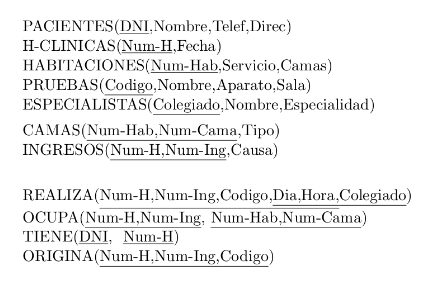
\includegraphics[width=0.8\textwidth]{images/1_3B.png}
        \caption{Ejercicio 1 de la relación 3 B.}
        \label{fig:ej1RelB}
    \end{figure}
    \begin{itemize}
        \item En Camas, la clave Num-Hab es clave externa a Habitaciones.
        \item En Ingresos, la clave Num-H es clave externa a H-Clínicas.
        \item En Realiza, las claves Num-H y Num-Ing son claves externas a Ingresos, y la clave Colegiado es clave externa a Especialistas.
        \item En Ocupa, las claves Num-H y Num-Ing son claves externas a Ingresos, y la clave Num-Hab es clave externa a Habitaciones.
        \item En Tiene, la clave Num-H es clave externa a H-Clínicasy DNI es clave externa a Pacientes.
        \item En Origina, las claves Num-H y Num-Ing son claves externas a Ingresos, y la clave Código es clave externa a Pruebas.
    \end{itemize}
    \item Atendiendo al siguiente diseño:
    \begin{figure}[H]
        \centering
        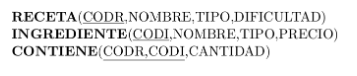
\includegraphics[width=0.5\textwidth]{images/ej2_1.png}
    \end{figure}
    El tipo de receta contempla: primero, segundo y postre, y el tipo de ingrediente es grano,
    liquido, polvo, troceado y otro. Indica la línea de las tuplas incorrectas y la regla de integridad
    que crees que viola.

    \begin{figure}[H]
        \centering
        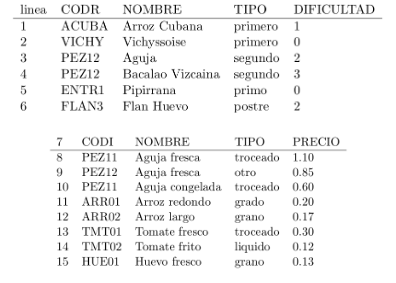
\includegraphics[width=0.5\textwidth]{images/ej2_2.png}
        \label{fig:ej2RelB}
    \end{figure}
    \begin{figure}[H]
        \centering
        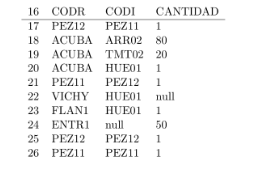
\includegraphics[width=0.5\textwidth]{images/ej2_3.png}
        \label{fig:ej2RelB2}
    \end{figure}
    \begin{itemize}
        \item Tupla 5 el tipo no aparece en los valores posibles.
        \item Tupla 3 y 4 se repite la CP (PEZ12).
        \item Tupla 8 y 10 se repite la CP (PEZ11).
        \item Tupla 11 el tipo no aparece en los valores posibles.
        \item Tupla 24 la CP es nula.
    \end{itemize}
    \item Sea el siguiente esquema de una BD de animales de un zoo:
    \begin{figure}[H]
        \centering
        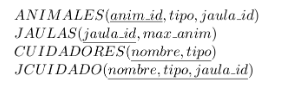
\includegraphics[width=0.5\textwidth]{images/ej3.png}
        \label{fig:ej3RelB}
    \end{figure}
    El atributo tipo en ANIMALES y CUIDADORES deben coincidir (lista enumerada).
    % \begin{itemize}
    %     \item Indicar las claves externas y a qué referencian.
    %     \item Muestra una instancia de cada relación con 4 tuplas en cada una.
    %     \item Introduce nuevas muestras para que se cumpla que una jaula es compartida por varios tipos de animales y que varios cuidadores pueden actuar de suplentes.
    %     \item Introduce una tupla en JCUIDADO tal que el cuidador no pueda atender a ningún animal de la jaula. ¿Está violando alguna regla de integridad?
    %     \item Introduce una tupla en JCUIDADO que viole la restricción de integridad referencial.
    % \end{itemize}
    %--------------------------Answer--------------------------
    \begin{itemize}
        \item El atributo tipo en ANIMALES y CUIDADORES deben coincidir (lista enumerada).
        \item Indicar las claves externas y a qué referencian:
        \begin{itemize}
            \item En JCUIDADO, \texttt{nombre}, \texttt{tipo} referencian \texttt{CUIDADORES}.
            \item En JCUIDADO, \texttt{jaula\_id} referencia a \texttt{JAULAS}.
        \end{itemize}
        \item Muestra una instancia de cada relación con 4 tuplas en cada una:
    \end{itemize}

    \begin{table}[h!]
    \centering
    \caption{ANIMALES}
    \begin{tabular}{|c|c|c|}
    \hline
    \textbf{anim\_id} & \textbf{tipo} & \textbf{jaula\_id} \\ \hline
    Tig              & Mamífero      & 1                  \\ \hline
    Leo              & Mamífero      & 2                  \\ \hline
    Koa              & Mamífero      & 3                  \\ \hline
    Jir              & Mamífero      & 3                  \\ \hline
    \end{tabular}
    \end{table}

    \begin{table}[h!]
    \centering
    \caption{JAULAS}
    \begin{tabular}{|c|c|}
    \hline
    \textbf{jaula\_id} & \textbf{max\_anim} \\ \hline
    1                  & 1                  \\ \hline
    2                  & 1                  \\ \hline
    3                  & 2                  \\ \hline
    4                  & 3                  \\ \hline
    \end{tabular}
    \end{table}

    \begin{table}[h!]
    \centering
    \caption{CUIDADORES}
    \begin{tabular}{|c|c|}
    \hline
    \textbf{nombre} & \textbf{tipo} \\ \hline
    Jose           & Mamífero      \\ \hline
    Pedro          & Pez           \\ \hline
    María          & Mamífero      \\ \hline
    Sara           & Mamífero      \\ \hline
    \end{tabular}
    \end{table}

    \begin{table}[h!]
    \centering
    \caption{JCUIDADO}
    \begin{tabular}{|c|c|c|}
    \hline
    \textbf{nombre} & \textbf{tipo} & \textbf{jaula\_id} \\ \hline
    Jose           & Mamífero      & 1                  \\ \hline
    María          & Mamífero      & 2                  \\ \hline
    Sara           & Mamífero      & 3                  \\ \hline
    Sara           & Mamífero      & 2                  \\ \hline
    \end{tabular}
    \end{table}
    \begin{itemize}
        \item Introduce nuevas muestras para que se cumpla que una jaula es compartida por varios tipos de animales y que varios cuidadores pueden actuar de suplentes:
        \begin{table}[h!]
        \centering
        \caption{ANIMALES (actualizado)}
        \begin{tabular}{|c|c|c|}
        \hline
        \textbf{anim\_id} & \textbf{tipo} & \textbf{jaula\_id} \\ \hline
        Tig              & Mamífero      & 1                  \\ \hline
        Leo              & Mamífero      & 2                  \\ \hline
        Koa              & Reptil        & 3                  \\ \hline
        Jir              & Mamífero      & 3                  \\ \hline
        \end{tabular}
        \end{table}

        \begin{table}[h!]
        \centering
        \caption{CUIDADORES (actualizado)}
        \begin{tabular}{|c|c|}
        \hline
        \textbf{nombre} & \textbf{tipo} \\ \hline
        Jose           & Mamífero      \\ \hline
        Pedro          & Reptil        \\ \hline
        María          & Mamífero      \\ \hline
        Sara           & Mamífero      \\ \hline
        \end{tabular}
        \end{table}

        \begin{table}[h!]
        \centering
        \caption{JCUIDADO (actualizado)}
        \begin{tabular}{|c|c|c|}
        \hline
        \textbf{nombre} & \textbf{tipo} & \textbf{jaula\_id} \\ \hline
        Jose           & Mamífero      & 1                  \\ \hline
        María          & Mamífero      & 2                  \\ \hline
        Sara           & Mamífero      & 3                  \\ \hline
        Pedro          & Reptil        & 3                  \\ \hline
        \end{tabular}
        \end{table}

        \item Introduce una tupla en JCUIDADO tal que el cuidador no pueda atender a ningún animal de la jaula. ¿Está violando alguna regla de integridad?  
        Sí, viola la regla de integridad referencial porque el tipo del cuidador no coincide con el tipo de los animales en la jaula.

        Ejemplo de tupla inválida:  
        \texttt{(Pedro, Reptil, 1)}.  
        Aquí, Pedro no puede atender a la jaula 1 porque contiene mamíferos.

        \item Introduce una tupla en JCUIDADO que viole la restricción de integridad referencial:  
        Ejemplo de tupla inválida:  
        \texttt{(Ana, Ave, 5)}.  
        Aquí, la jaula 5 no existe en la tabla JAULAS, lo que viola la integridad referencial.
    \end{itemize}
\end{enumerate}